% !TEX root = ../main.tex

\chapter{评估}

\section{评估设置}

我们使用四种广泛采用的指标对模型进行评估:Fréchet Gesture Distance(FGD)\cite{speech_gesture_generation}、L1 动作多样性(L1DIV)\cite{beatcamn}、节奏对齐度(Beat Alignment, BA)\cite{beatcamn},以及语义相关动作召回率(SRGR)\cite{beatcamn}。所有评估均在 BEAT 数据集上进行,选用说话人编号为 2、4、6 和 8。生成的身体姿态与真实标签均采用相同骨架拓扑的 BVH 格式。FGD 特征由 EMAGE 模型 \cite{emage} 提取,L1DIV、BA 和 SRGR 的实现使用 BEAT 官方提供的代码。所有指标在四位说话人上取平均,以减少个体差异带来的偏差。

\section{客观评估指标与实现细节}
\label{sec:objective_metrics}

为全面评价模型在动作自然性、节奏同步性与多样性等方面的表现,
本文在客观指标层面采用四项度量:Fréchet Gesture Distance (FGD)、Speech–Gesture Rhythm Correlation (SRGR)、Beat Alignment (BA) 以及 L1-based Diversity (L1DIV)。
这些指标分别对应生成动作在分布一致性、语音同步性与变化丰富性等不同维度,
共同构成对模型质量的综合评估体系。

其中,FGD 作为生成分布的核心统计指标,需要训练额外的动作自编码器(AutoEncoder, AE)作为特征提取器;
其余指标则直接基于生成序列与语音信号的时间对应关系进行计算。
本节首先介绍 FGD 的计算原理与评估模型结构,
随后依次阐述其它三项指标的定义与计算方法。

\subsection{Fréchet Gesture Distance (FGD)}
\label{subsec:fgd}

FGD\cite{speech_gesture_generation}用于衡量生成手势分布与真实手势分布之间的统计距离,
灵感源自图像生成领域的 Fréchet Inception Distance (FID)。
不同于图像任务直接利用 Inception 网络特征,
在动作生成领域,特征空间需由单独训练的动作自编码器定义。
该自编码器通过重构任务学习手势的潜在表示,使潜在空间具备对运动模式的压缩与区分能力。
在该潜在空间中,假设真实分布与生成分布的高维嵌入向量分别为
$\mathcal{N}(\bm{\mu}_r, \bm{\Sigma}_r)$ 与 $\mathcal{N}(\bm{\mu}_g, \bm{\Sigma}_g)$,
则 FGD 定义为:
\begin{equation}
\mathrm{FGD} = 
\|\bm{\mu}_r - \bm{\mu}_g\|_2^2 +
\mathrm{Tr}(\bm{\Sigma}_r + \bm{\Sigma}_g - 2(\bm{\Sigma}_r \bm{\Sigma}_g)^{1/2}).
\end{equation}

较小的 FGD 值表示生成动作的统计分布更接近真实数据,
可反映动作的整体自然度与风格一致性。

\paragraph{评估模型结构与训练配置.}
本文在每位说话人的训练集上分别训练一组评估用自编码器,以避免跨说话人分布差异对指标的干扰。
自编码器输入为以 Rot6d 表示的上半身骨架序列,
训练目标为最小化位置、速度与加速度的多尺度重构误差:
\begin{equation}
\mathcal{L}_{AE} = 
\|\hat{\bm{g}} - \bm{g}\|_2^2 +
\lambda_v \|\hat{\bm{g}}' - \bm{g}'\|_2^2 +
\lambda_a \|\hat{\bm{g}}'' - \bm{g}''\|_2^2,
\end{equation}
其中 $\lambda_v = 0.1$, $\lambda_a = 0.1$,$\bm{g}'$、$\bm{g}''$分别为速度与加速度序列。

训练配置如下:
输入片段长度为 32 帧,批大小 256,隐藏层维度 128,学习率 $1.2\times10^{-4}$,优化器为 Adam;
共训练 400 轮。
训练片段步长设为 10,以增加样本数量并保持时间连续性。

\paragraph{骨架拓扑敏感的自编码器.}
在基线模型 CaMN 的 FGD 评估中,使用了基于时间卷积的平铺向量编码器(Embedding-based AutoEncoder)。
该结构将整帧姿态作为高维向量输入,对旋转参数的数值尺度高度敏感,
当使用 Rot6d 表示时,各关节分量的方差差异会在潜在空间中被放大,
导致潜在分布协方差矩阵奇异,从而引起 FGD 数值爆炸。

为避免此问题,本文采用基于骨架拓扑卷积的自编码器(Skeleton-aware AutoEncoder)作为 FGD 特征提取器。
该模型在编码层中引入骨架邻接矩阵 $A$,
通过局部卷积核在相邻关节之间共享权重:
\begin{equation}
\mathbf{h}_i^{(l+1)} = 
\sigma\left(
\sum_{j \in \mathcal{N}(i)} A_{ij} W^{(l)} \mathbf{h}_j^{(l)} + b^{(l)}
\right),
\end{equation}
从而在空间上实现局部归一与结构平滑。
这一设计使特征提取对旋转表示形式不敏感,
可在欧拉角、Axis-Angle 与 Rot6d 等不同表示下保持稳定的潜在分布。
在本文的实验中,该结构显著提高了 FGD 的鲁棒性,
避免了 EmbeddingNet 评估器在 Rot6d 表示下协方差爆炸的现象。

\paragraph{指标计算流程.}
在获得评估模型后,
分别将生成序列与真实序列输入自编码器的编码器部分,
提取潜在特征 $\bm{z}_g$ 与 $\bm{z}_r$,
再计算两者的均值与协方差以求得 FGD。
评估时按说话人独立计算,再取平均值作为总体指标。

\subsection{Speech–Gesture Rhythm Correlation (SRGR)}
\label{subsec:srgr}

SRGR 指标\cite{beatcamn}用于衡量生成手势与语音韵律在节奏层面的同步性,
其核心思想是比较语音能量包络与手势运动速度包络的时间相关程度。
与整句级语义匹配不同,SRGR 反映的是语音与手势在局部时间尺度上的节奏耦合强度。

\paragraph{定义与原理.}
设语音能量序列为 $\bm{e} = \{ e_t \}$,
通过对语音短时能量(Short-Time Energy, STE)进行平滑得到;
手势运动速度定义为各关节旋转向量的一阶差分模长的平均值:
\begin{equation}
v_t = \frac{1}{J}\sum_{j=1}^{J} \|\bm{r}_{t,j} - \bm{r}_{t-1,j}\|_2,
\end{equation}
其中 $J$ 为关节数量,$\bm{r}_{t,j}$ 为第 $j$ 个关节在帧 $t$ 的旋转向量。

对两条时间序列 $\bm{e}$ 与 $\bm{v}$ 进行标准化后,
定义其皮尔逊相关系数(Pearson Correlation)为:
\begin{equation}
\mathrm{SRGR} = \frac{\mathrm{Cov}(\bm{e}, \bm{v})}{\sigma_{\bm{e}}\sigma_{\bm{v}}}.
\end{equation}
SRGR 值越高,表示手势运动节奏与语音节奏的同步程度越强,
通常取值范围在 $[-1, 1]$。
在实际实验中,为减少局部异常的影响,
本文在 1.5 秒滑动窗口内计算局部相关系数并取平均作为最终结果。

\paragraph{计算流程.}
1. 对语音信号计算短时能量,采用窗口长度 50\,ms、步长 10\,ms;  
2. 对生成与真实手势分别计算全身平均运动速度曲线;  
3. 将两条曲线统一至相同时间分辨率并进行归一化;  
4. 滑动计算局部皮尔逊相关系数,最后取平均值作为 SRGR。

该指标能客观反映模型在语音驱动节奏一致性方面的表现,
在主观实验中也与“同步性”评分显著相关。

\subsection{Beat Alignment (BA)}
\label{subsec:ba}

BA(Beat Alignment)指标\cite{beatcamn}用于衡量手势关键动作与语音重读节拍的时间对齐程度,
反映模型在\textbf{时序同步性(temporal synchronization)}方面的性能。
与 SRGR 的全局相关性不同,BA 更注重\textbf{事件级的对齐精度}。

\paragraph{定义与原理.}
设语音节拍集合为 $\mathcal{B}_s = \{t^s_k\}$,
通过检测语音短时能量或梅尔倒谱系数(MFCC)的局部峰值得到;
手势峰集合为 $\mathcal{B}_g = \{t^g_m\}$,
定义为手势速度 $v_t$ 的局部极大点集合。
对于每个语音节拍 $t^s_k$,
计算其最近手势峰的时间差 $\Delta t_k = \min_m |t^s_k - t^g_m|$。
则 BA 指标定义为:
\begin{equation}
\mathrm{BA} = 1 - \frac{1}{K} \sum_{k=1}^{K} \frac{\Delta t_k}{\tau},
\end{equation}
其中 $K$ 为节拍数,$\tau$ 为允许最大偏差阈值(本文取 $\tau=0.5$\,s)。
当 $\Delta t_k < \tau$ 时,记为一次成功对齐。
因此 $\mathrm{BA}$ 越接近 1,表明手势动作越能准确响应语音重读节拍。

\paragraph{计算流程.}
1. 通过能量包络峰值检测获取语音节拍点;  
2. 通过运动速度极值检测获取手势关键帧;  
3. 计算两者的最短时间偏差并归一化;  
4. 平均所有节拍对齐率,得到整体 BA 指标。  

本文使用该指标评估模型在节奏突变与强调语气时的响应能力。
在主观观察中,BA 与视觉上“语音同步自然度”呈正相关。

\subsection{L1-based Diversity (L1DIV)}
\label{subsec:l1div}

L1DIV 指标\cite{beatcamn}衡量生成手势序列的多样性(diversity),
即不同语音输入下模型生成结果的动作差异程度。
该指标反映模型在保持自然性的同时,
能否避免生成收敛到平均动作模式(mode collapse)的倾向。

\paragraph{定义与原理.}
设模型对同一语音片段的 $N$ 次生成结果为
$\{\bm{g}^{(1)}, \bm{g}^{(2)}, \dots, \bm{g}^{(N)}\}$,
则 L1 多样性定义为任意两序列间平均 L1 距离:
\begin{equation}
\mathrm{L1DIV} = 
\frac{2}{N(N-1)} \sum_{i<j} 
\frac{1}{T} \sum_{t=1}^{T} 
\|\bm{g}^{(i)}_t - \bm{g}^{(j)}_t\|_1.
\end{equation}
当 $N=2$ 时,该指标即为两次独立生成的平均动作差异。

\paragraph{计算流程.}
1. 对同一语音输入重复生成多次(不同随机噪声或 dropout 路径);  
2. 对每帧姿态计算关节旋转的 L1 差;  
3. 对时间与样本求平均得到整体 L1DIV 值。  

较高的 L1DIV 表明模型生成具有较强的多样性,
但过高可能意味着动作不稳定或噪声放大。
因此,L1DIV 通常与 FGD 联合分析:  
FGD 反映真实度,L1DIV 反映丰富度,
两者共同平衡模型在自然性—多样性维度上的表现。

\section{模型对比概览}

表~\ref{tab:modalitycomparison} 总结了各模型的输入输出模态特征。值得注意的是,我们的模型是唯一同时支持“头部姿态”输入且完全不依赖未来信息的方案。

\begin{table}[h]
\centering
\resizebox{\linewidth}{!}{%
\begin{tabular}{@{}lccccc|c|c@{}}
\toprule
\multirow{2}{*}{模型} & \multicolumn{5}{c|}{输入模态} & \multirow{2}{*}{未来信息} & \multirow{2}{*}{输出} \\ 
\cmidrule(lr){2-6}
 & 音频 & 面部捕捉 & 头部姿态 & 说话人ID & 情绪 &  &  \\ 
\midrule
CaMN       & $\checkmark$ & $\checkmark$ & $\times$ & $\checkmark$ & $\checkmark$ & $\checkmark$ & 身体 \\
DiffSHEG   & $\checkmark$ & $\times$ & $\times$ & $\checkmark$ & $\times$ & $\checkmark$ & 身体+面部 \\
本方法     & $\checkmark$ & $\checkmark$ & $\checkmark$ & $\ast$ & $\times$ & $\times$ & 身体 \\ 
\bottomrule
\end{tabular}%
}

\section{用户调研}
\label{sec:userstudy}

为进一步验证模型在真实交互环境中的表现,
本文进行了用户主观评估实验,
比较 FaceCapGes、DiffSHEG \cite{diffsheg} 与 CaMN \cite{beatcamn} 三个模型在动作自然性、同步性与多样性方面的主观质量。
本节首先介绍用户研究系统与实验配置,
随后报告主观评价结果与分析。

\subsection{评估系统与实验配置}

\paragraph{实验材料与呈现方式.}
用户评估所使用的手势动画均基于测试集语音片段生成,
并以BVH(Biovision Hierarchy)文件形式保存。
BVH 是一种通用的动作捕捉数据格式,
通过层级化定义骨骼结构与帧级旋转参数,
可直接导入 3D 动画与虚拟人系统。
本文使用的 BVH 文件采用欧拉角旋转表示,以保证与 Unity 的骨骼系统兼容。

由于三种对比模型的输出旋转参数形式不同——
CaMN 模型直接输出欧拉角,
DiffSHEG 输出 Axis-Angle,
而 FaceCapGes 输出 Rot6d 表示——
因此在导出 BVH 之前,
需将后两者统一转换为欧拉角表示,
以便在同一骨架拓扑下进行动画比较。

所有对比模型(FaceCapGes、CaMN、DiffSHEG)均使用相同的训练集与骨骼定义,
其中 CaMN 与 DiffSHEG 采用各自论文公开的原版参数。
虚拟人角色选自 BEAT 数据集提供的公开演讲者模型集合,
并经过 Unity 的 Mecanim 自动骨骼绑定系统匹配。
该系统会自动配对 BVH 文件中定义的骨骼层级与虚拟人模型的骨骼节点,
从而在不依赖手动权重绘制的情况下完成动作重定向。

本系统当前支持的虚拟人模型需同时具备骨骼绑定与 ARKit 兼容的 BlendShape 参数。
基于此约束,实验选用了 CaMN 论文公开的男女两名演讲者模型,二者均满足兼容要求,可实现身体与面部的联合驱动。

\paragraph{播放系统实现.}
我们基于 Unity 自行编写播放脚本,
将各模型生成的 BVH 动画用于驱动虚拟人身体骨骼,
同时以面部捕捉序列驱动 BlendShape 表情参数,
并同步播放原始语音音频。
系统支持同时呈现三种模型生成的动画结果:
用户可在同一画面中(左、中、右)并行观察三种手势表现,
所有语音与面部表情完全一致,
唯一变量为身体动作。
该设计使参与者能够直接比较不同模型在动作风格、
节奏响应与语音同步性方面的差异。

为确保主观评价的公正性与可重复性,
系统在每次实验开始前会随机分配三种模型的位置(左、中、右),
界面上不会显示模型名称,
从而避免潜在偏向。
各测试片段的播放顺序在实验前统一设定,
以保证不同参与者之间的样本顺序均衡。
实验员在播放系统后台记录当前序列与模型对应关系,
以便后续结果统计。

\paragraph{实验界面与设备.}
评估系统提供桌面端与 VR 端两种版本,功能完全一致。
VR 版本基于 PICO 设备实现;
桌面版支持多窗口并行播放,方便用户同时对比。
如图~\ref{fig:userstudy_app} 所示,
播放界面在两种设备上保持统一布局,
播放完成后参与者需通过交互界面对三个模型进行排序打分。
VR 用户在沉浸式环境中逐一观看三段动画;
桌面端用户则可在单屏上同时观察全部模型。
因此前者注重细节感知与临场性,
后者更有利于整体风格与节奏的一致性对比。

\paragraph{实验流程与指导.}
实验正式开始前,
研究人员向参与者说明了三项主观评价标准的含义,
确保所有被试对评分维度理解一致:
\begin{itemize}
    \item \textbf{真实感(Realism)}:整体动作是否自然流畅,是否存在明显的违和感,如朝向异常或突然抖动;
    \item \textbf{同步性(Synchronization)}:手势动作与语调、语音节奏是否协调一致;
    \item \textbf{多样性(Diversity)}:手势是否丰富多变,避免长时间静止或重复单一动作。
\end{itemize}

在实验过程中,
VR 版本于\textbf{线下环境}进行,
桌面版通过\textbf{线上远程环境}执行。
两种形式均保持实时交流通道,
研究人员可在参与者提问时即时解释操作或澄清评分标准。
在正式评估阶段,
参与者可多次重播当前片段,
但不能返回查看先前内容,
以减少记忆偏差。
所有播放条件(\textbf{Unity 场景内的相机角度、光照参数、音量与分辨率设置})
在全部被试中保持一致,
以确保渲染输出的可比性。

需要说明的是,
对于\textbf{VR 实验},
所有测试均在相同的线下实验室环境中进行,
使用同一套 PICO 设备与照明条件;
而\textbf{桌面端实验}通过远程方式执行,
参与者在各自电脑上运行实验程序。
研究人员可通过实时屏幕共享观察其操作流程并保持语音沟通,
但无法严格控制其所在房间的光照或环境噪声条件。
因此,桌面端实验在“观看环境”上存在一定差异,
但由于任务内容与播放系统完全相同,
且实验员在测试中持续指导,
可认为该差异对结果的总体影响有限。

\paragraph{实验材料与任务设计.}
评估样本来自 BEAT 数据集中四位演讲者(ID 2、4、6、8),
其中 2、4 为男性,6、8 为女性。
每位演讲者各选取两段平均长度约 1 分钟的语音片段,
演讲话题互不重复,共组成 \textbf{8 段固定视频样本}。
所有实验均使用相同的 8 段样本,
但其\textbf{呈现顺序在不同被试间经过随机化或平衡化处理},
以避免顺序效应(order effect)。
每段视频均包含三种模型生成的动作版本(FaceCapGes、CaMN、DiffSHEG),
并在播放时随机分配其在屏幕的左右位置。
参与者在观看每个片段后,
根据三项主观标准(真实感、同步性、多样性)
对三个模型的表现进行排序评估。

\begin{figure}[h!t]
\centering
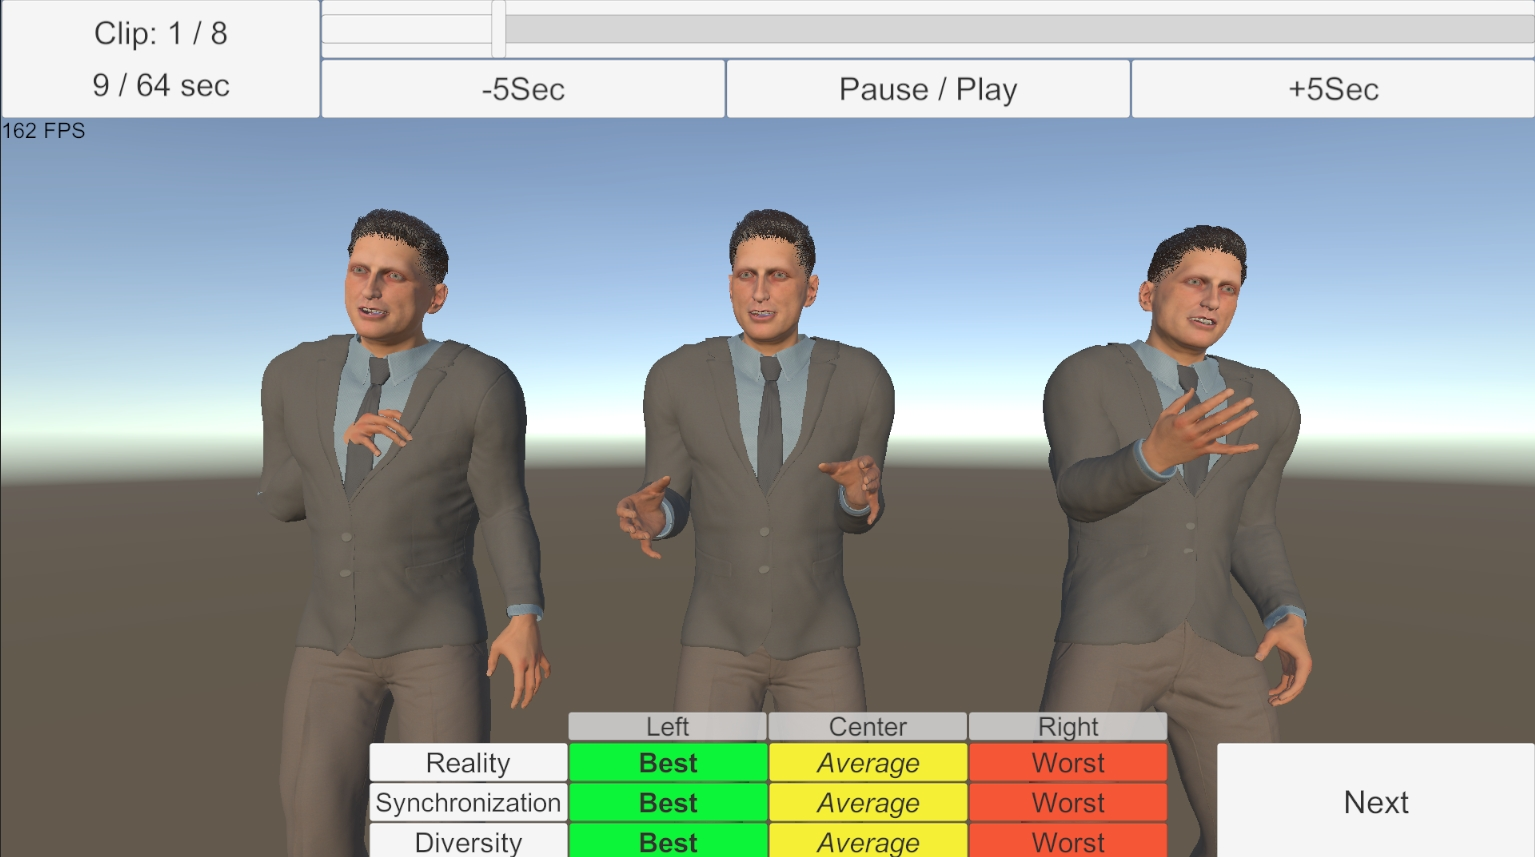
\includegraphics[width=\linewidth]{figures/UserStudyImage.png}
\caption{用户研究系统界面示意图。
左、中、右位置随机分配给三种模型,
音频与面部表情完全一致,仅身体动作不同。}
\label{fig:userstudy_app}
\end{figure}

\paragraph{实验参与者.}
共邀请 16 名参与者(12 名使用 VR 设备,4 名使用桌面端),
涵盖不同性别与学术背景。
所有参与者在实验前均接受了操作说明与校准,
并在系统指导下完成评分练习。
为避免呈现顺序对主观印象造成偏差,
另设计了采用平衡拉丁方(Balanced Latin Square)顺序的实验版本,
使不同参与者观看样本的顺序均衡分布。

\subsection{平衡拉丁方排序设计}
\label{subsec:latin_square}

该版本实验共招募 8 位 VR 用户(4 男 4 女),
排序顺序由 HCI 用户研究工具包 \cite{LatinSquareToolkit} 自动生成,
确保模型与演讲者组合的呈现顺序在全体被试间均匀分布。
所有条件保持一致,唯一变量为视频播放顺序。

\subsection{结果与分析}
\label{subsec:user_study_result}

本节综合分析两轮用户评估的统计结果与参与者反馈。
所有结果均基于相同的 8 段测试样本,
其中模型位置与播放顺序在不同被试间随机化或经平衡拉丁方控制,
以保证主观评价的公正性。

\paragraph{电脑用户测评结果.}
如图~\ref{fig:userstudy} 所示,
在 16 名参与者的总体评价中,
FaceCapGes 在三个维度(真实感、同步性、多样性)上均优于基线模型 CaMN,
并在“真实感”方面与离线扩散模型 DiffSHEG 持平。
这一结果表明,FaceCapGes 虽在严格的实时因果约束下运行,
但仍能保持与非实时生成模型相近的动作自然度与流畅性。

\begin{figure}[h!t]
\centering
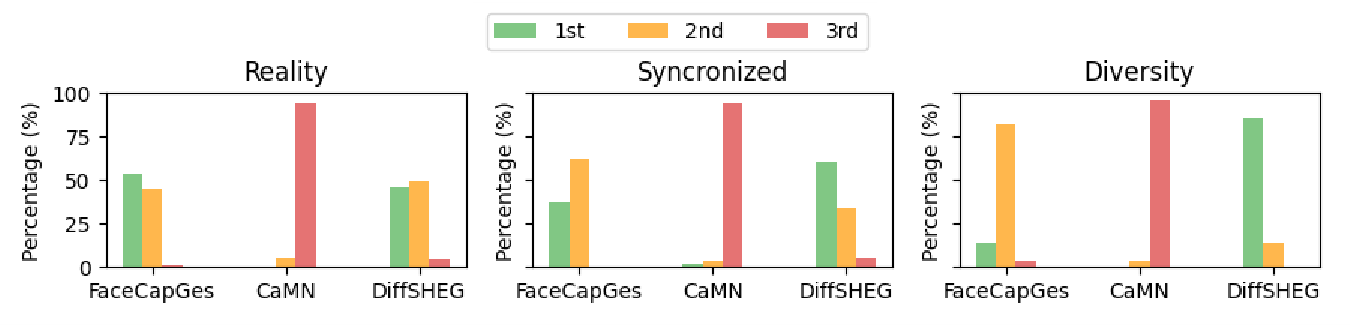
\includegraphics[width=\linewidth]{figures/UserStudy_All.png}
\caption{16 名参与者对三种模型在“真实感”、“同步性”和“多样性”三个维度的主观排名结果。}
\label{fig:userstudy}
\end{figure}

\paragraph{平衡拉丁方实验结果.}
图~\ref{fig:userstudy_latin_square} 展示了平衡拉丁方实验版本中 8 位 VR 用户的独立结果,
该版本严格控制了模型与演讲者组合的呈现顺序。
结果与总体趋势一致,
FaceCapGes 在“同步性”与“真实感”上显著优于 CaMN,
并在“多样性”指标上与 DiffSHEG 接近。
这表明实验结果在不同顺序条件下保持稳定,
进一步验证了模型在多维度主观评价中的一致优势。

\begin{figure}[h!t]
\centering
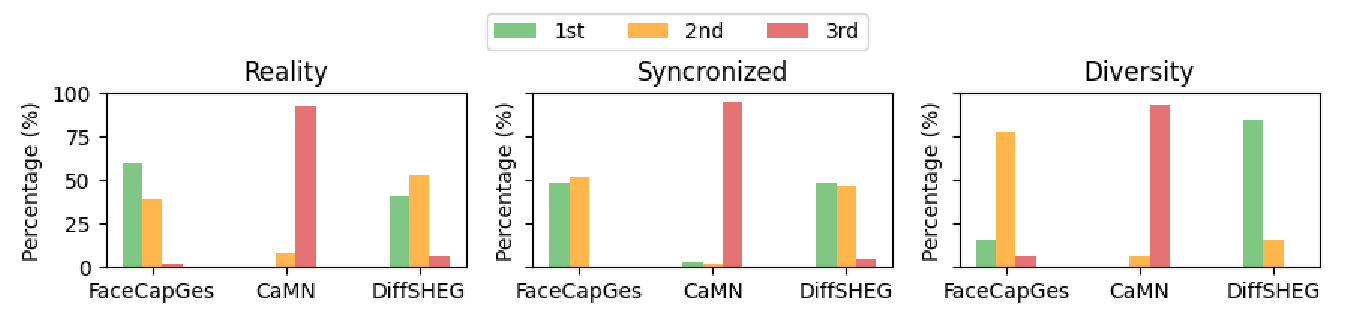
\includegraphics[width=\linewidth]{figures/UserStudy_LatinSquare.png}
\caption{平衡拉丁方实验版本中 8 位 VR 用户的主观排名结果,
评价维度包括“真实感”、“同步性”和“多样性”。}
\label{fig:userstudy_latin_square}
\end{figure}

\paragraph{用户反馈分析.}
根据实验后访谈与自由评论汇总,
参与者普遍认为 FaceCapGes 的动作过渡自然、节奏感强,
手势响应与语音重音、语调变化更加一致。
部分 VR 用户指出,
在沉浸式视角下能够明显感受到手势的连贯性与时序协调,
而 CaMN 在头部与上身动作衔接处偶有“僵硬”或“转向延迟”现象。
约三分之一的参与者提到 DiffSHEG 的动作表现力最强,
但在某些片段中出现手部摆动幅度过大或抖动的情况,
导致同步性评分略低。

桌面端用户普遍认为三种模型的差异在节奏与流畅性上最明显;
VR 用户则更容易察觉动作的空间一致性与临场协调。
两组被试的整体排序趋势一致,
说明模型差异具有跨设备一致性。

\paragraph{结果讨论.}
CaMN 得分较低的主要原因在于其采用欧拉角表示,
导致部分姿态序列在旋转空间中出现不连续,
尤其在头部动作上易产生跳变;
而 DiffSHEG 的高方差输出虽提升了动作多样性,
但表现出一定的突然颤抖,可能来源于Axis-Angle的不连续性。
相比之下,
FaceCapGes 的因果式时间建模和头部姿态融合策略
有效提升了局部动作的平滑性与节奏协调,
使其在实时条件下同时兼顾自然度与稳定性。
此外,
实验的平衡拉丁方版本进一步证明结果在不同呈现顺序下的一致性,
排除了顺序偏差对主观评价的显著影响。

综上,
用户研究表明 FaceCapGes 在实时生成条件下
仍能维持与离线模型相当的主观表现,
在动作真实感、节奏同步性和长时间交互稳定性方面
均显著优于传统因果结构基线,
验证了本文提出的多模态融合与时间建模策略的有效性。

\section{定性分析}

我们强烈建议观看电子附录中的演示视频,内容包含 GT、CaMN、DiffSHEG 与本模型的并排展示,能够直观体现时间对齐性、手势响应性以及头-身协调性方面的差异。

如图~\ref{fig3} 所示,FaceCapGes 能平滑且富有表现力地捕捉说话人动态。与 CaMN 相比,本模型避免了欧拉角带来的不连续问题,生成的身体动作可顺应头部运动趋势。与 DiffSHEG 相比,我们的模型在动作速度上略逊一筹,但能有效避免抖动或夸张姿态。头部姿态的引入也明显提升了手势方向与语义的一致性。

\begin{figure*}[h!t]
\centering
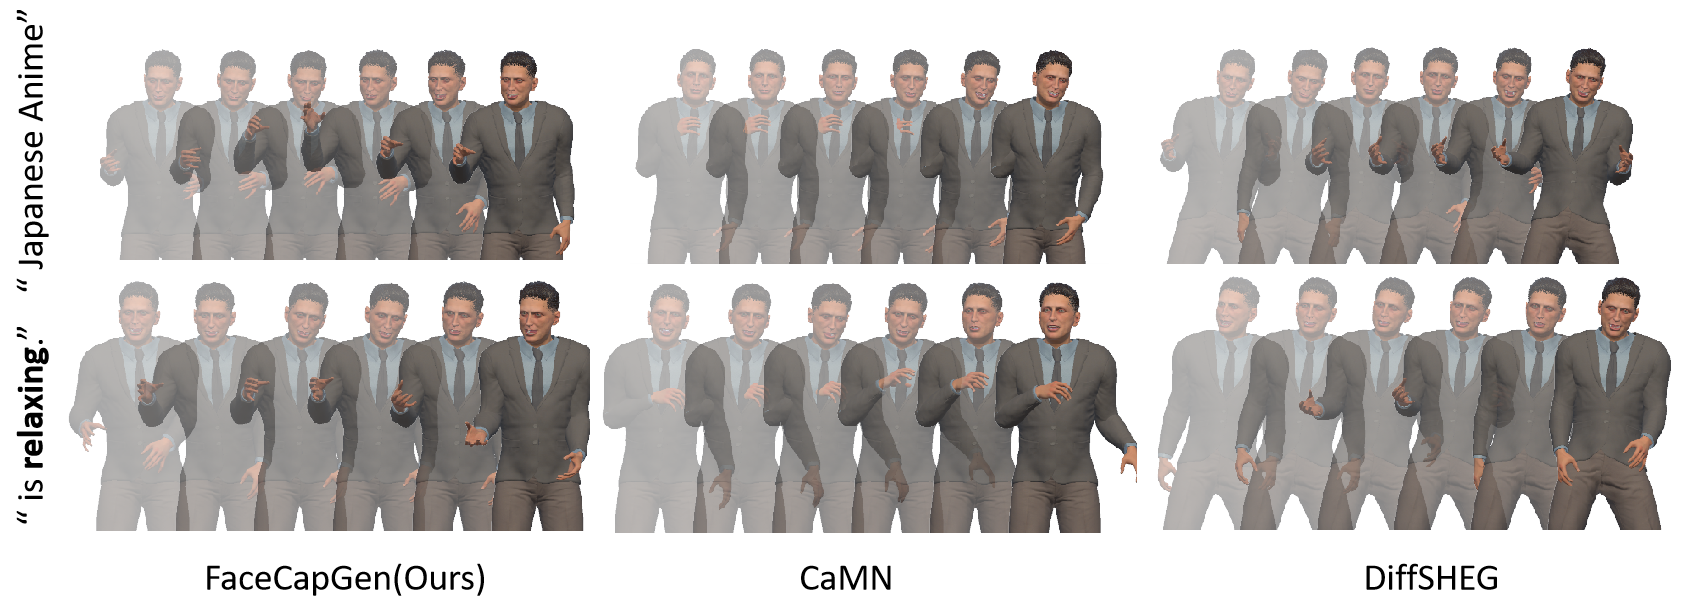
\includegraphics[width=\textwidth]{figures/GeneratedPoseOverview.png}
\caption{GT、CaMN、DiffSHEG 与 FaceCapGes 的动作效果对比。本模型手势响应自然,方向与头部朝向一致。}
\label{fig3}
\end{figure*}

\section{定量分析}

\begin{table*}[h]
\centering
\begin{tabular}{@{}lclrrrr@{}}
\hline
区域 & 方法 & FGD\textdownarrow & SRGR\textuparrow & BA\textuparrow & L1DIV\textuparrow \\
\hline
\multirow{3}{*}{全身}
& CaMN       & 47.732 & 0.098 & 0.845 & 7.591 \\
& DiffSHEG   & \underline{26.846} & \textbf{0.109} & \underline{0.883} & \underline{11.028} \\
& 本方法     & \textbf{23.385} & \underline{0.107} & \textbf{0.913} & \textbf{13.284} \\
\hline
\multirow{3}{*}{不含头部}
& CaMN       & 49.437 & 0.103 & 0.845 & 7.327 \\
& DiffSHEG   & \underline{26.847} & \textbf{0.110} & \underline{0.883} & \underline{10.990} \\
& 本方法     & \textbf{23.384} & \underline{0.107} & \textbf{0.913} & \textbf{13.330} \\
\hline
\end{tabular}
\caption{在 BEAT 四位说话人测试集上的定量评估结果。FaceCapGes 在所有指标上优于 CaMN,且与 DiffSHEG 表现相当。}
\label{tab1}
\end{table*}

表~\ref{tab1} 显示,FaceCapGes 在所有指标上均优于 CaMN。与 DiffSHEG 相比,本模型 FGD 更低,SRGR 相近,且在 L1DIV 上表现最优,表明其生成动作具备良好多样性。但这一结论与用户主观评分存在一定出入:DiffSHEG 在“多样性”上主观排名更高。

这一差异揭示了 L1DIV 的局限性:它主要衡量空间偏离程度,并不能体现动作频率或视觉表现力。虽然我们的模型在结构上更丰富,但用户普遍认为 DiffSHEG 更“活跃”,吸引注意。这说明 L1DIV 无法完全捕捉感知上的丰富性,进一步强调定量与主观评估的互补作用。

\section{消融实验分析}

\begin{table*}[h]
\centering
\begin{tabular}{@{}llrrrr@{}}
\hline
区域 & 变体 & FGD\textdownarrow & SRGR\textuparrow & BA\textuparrow & L1DIV\textuparrow \\
\hline
\multirow{4}{*}{全身}
& CaMN                    & 32.870  & 0.111  & 0.858  & 7.214  \\
& 移除头部姿态           & 19.591  & 0.123  & 0.916  & 10.642 \\
& 移除帧级生成           & 21.592  & \textbf{0.125}  & 0.892  & 10.456 \\
& FaceCapGes(本方法)   & \textbf{19.290}  & 0.123 & \textbf{0.918}  & \textbf{10.871} \\
\hline
\end{tabular}
\caption{说话人 2 的消融实验结果。头部姿态对提升手势自然性与表达力有显著作用。}
\label{tab2}
\end{table*}

表~\ref{tab2} 展示了各模块对模型性能的影响。移除头部姿态会导致所有指标下降,证明其对表达性手势的重要性。

值得注意的是,“非帧级”版本使用未来上下文与双向 LSTM,但其表现反而不及帧级版本。这是因为它采用一次性解码,对每段输入独立处理,无法保证时间连续性,与原 CaMN 的设计一致。而我们的方法通过滑动窗口训练和自回归推理,逐帧依赖历史信息,使动作更连贯、过渡更自然。即使不使用未来帧,也能获得更低的 FGD 和更自然的手势对齐。

\section{性能评估}

\begin{table}[h]
\centering
\begin{tabular}{@{}lr@{}}
\hline
指标 & 时间 \\
\hline
测试帧数 & 93015 (f) \\
推理总时长 & 504 (s) \\
平均单帧时间 & 6.07E-03 (s/f) \\
\hline
\end{tabular}
\caption{在 RTX 4090 上的帧级推理速度评估结果。}
\label{tab3}
\end{table}

为评估实时性能,我们在 BEAT 测试集上使用 batch size 为 1 的配置进行推理测量。如表~\ref{tab3} 所示,模型平均每帧处理时间小于 7 毫秒,满足实时响应需求。

尽管模型推理本身较快,但系统总延迟还受输入特征提取影响。在我们的原型中,音频特征通过 Librosa 离线提取,93,015 帧总计耗时约 61 秒,单帧不足 1 毫秒。实际部署中可替换为如 PyAudio 或 SoundDevice 的实时提取方法,尽管本文未测量其具体延迟。

ARKit 面部追踪的延迟由开发文档估算约为 60FPS \cite{AppleARKitTrackingGuide}。结合模型推理时间,整体系统延迟预计不超过 25ms,足以满足实时虚拟人交互的需求。
